% 村松先生との打ち合わせ（2026年11月2日 9:00，オンライン）の資料．送らない（画面共有用）．
% ビルド: lualatex slides_1102_muramatsu.tex（2回）．規則: CLAUDE.md「Slides, notes and other documents」
% （私，，．，内部の番号を書かない，Abaqus は慶應での続きとしてのみ，記号は論文どおり，付録に記号と式）．
\documentclass[aspectratio=169,11pt]{beamer}
\usepackage{luatexja}
\usetheme{Madrid}
\usecolortheme{seahorse}
\usepackage{booktabs}
\usepackage{amsmath,amssymb}
\usepackage{xcolor}
\usepackage{graphicx}
\graphicspath{{../../assets/}{../../papers/coupling_paper/}}

\definecolor{c3}{RGB}{30,80,160}
\definecolor{cwarn}{RGB}{190,110,20}
\setbeamercolor{frametitle}{bg=c3, fg=white}
\setbeamertemplate{navigation symbols}{}

\title{修士論文の進捗と来年度の相談}
\subtitle{村松先生との打ち合わせ}
\author[西岡佳祐]{西岡佳祐}
\institute[IKM, LUH / 慶應]{%
\small ライプニッツ大学ハノーファー 連続体力学研究所（IKM）\\
\small 慶應義塾大学}
\date{2026年11月2日}

\begin{document}
\maketitle

% --------------------------------------------------------
\begin{frame}{今日の内容}
\begin{columns}[T]
\column{0.48\textwidth}
\textbf{報告}
\begin{enumerate}\setlength{\itemsep}{6pt}
  \item 修士論文の状況と日程
  \item 第4章の新しい結果（オリバーと合意した連成）
  \item 慶應での研究計画（本命の論文）
\end{enumerate}
\column{0.48\textwidth}
\textbf{ご相談}
\begin{enumerate}\setlength{\itemsep}{6pt}
  \item 来年の学会発表（USNCCM19，SQAI-NCTS）
  \item 4月からの RA
  \item 課題研究報告と慶應での修士論文
\end{enumerate}
\end{columns}
\end{frame}

% --------------------------------------------------------
\begin{frame}{修士論文の状況と日程}
\begin{itemize}\setlength{\itemsep}{6pt}
  \item 11月4日に本文を仕上げます．それまでに出た結果だけを使い，その後は足しません．
  \item 12月14日に PDF を Soleimani 先生へ提出し，12月16日 13:00 にコロキウム（IKM，対面，発表20分）．
  \item 1月に帰国します．
\end{itemize}
\vspace{6pt}
\begin{tabular}{ll}
\toprule
章 & 内容 \\
\midrule
第3章 & 5菌種の点モデルのベイズ較正（実測データ，確定済み）\\
第4章 & 成長則を IKM の要素へ実装・検証，点モデルを各 Gauss 点で連成（今回の更新）\\
第6章 & 結論，限界，慶應での続き \\
\bottomrule
\end{tabular}
\end{frame}

% --------------------------------------------------------
\begin{frame}{第4章：オリバーと合意した連成（10月20日）}
\centering
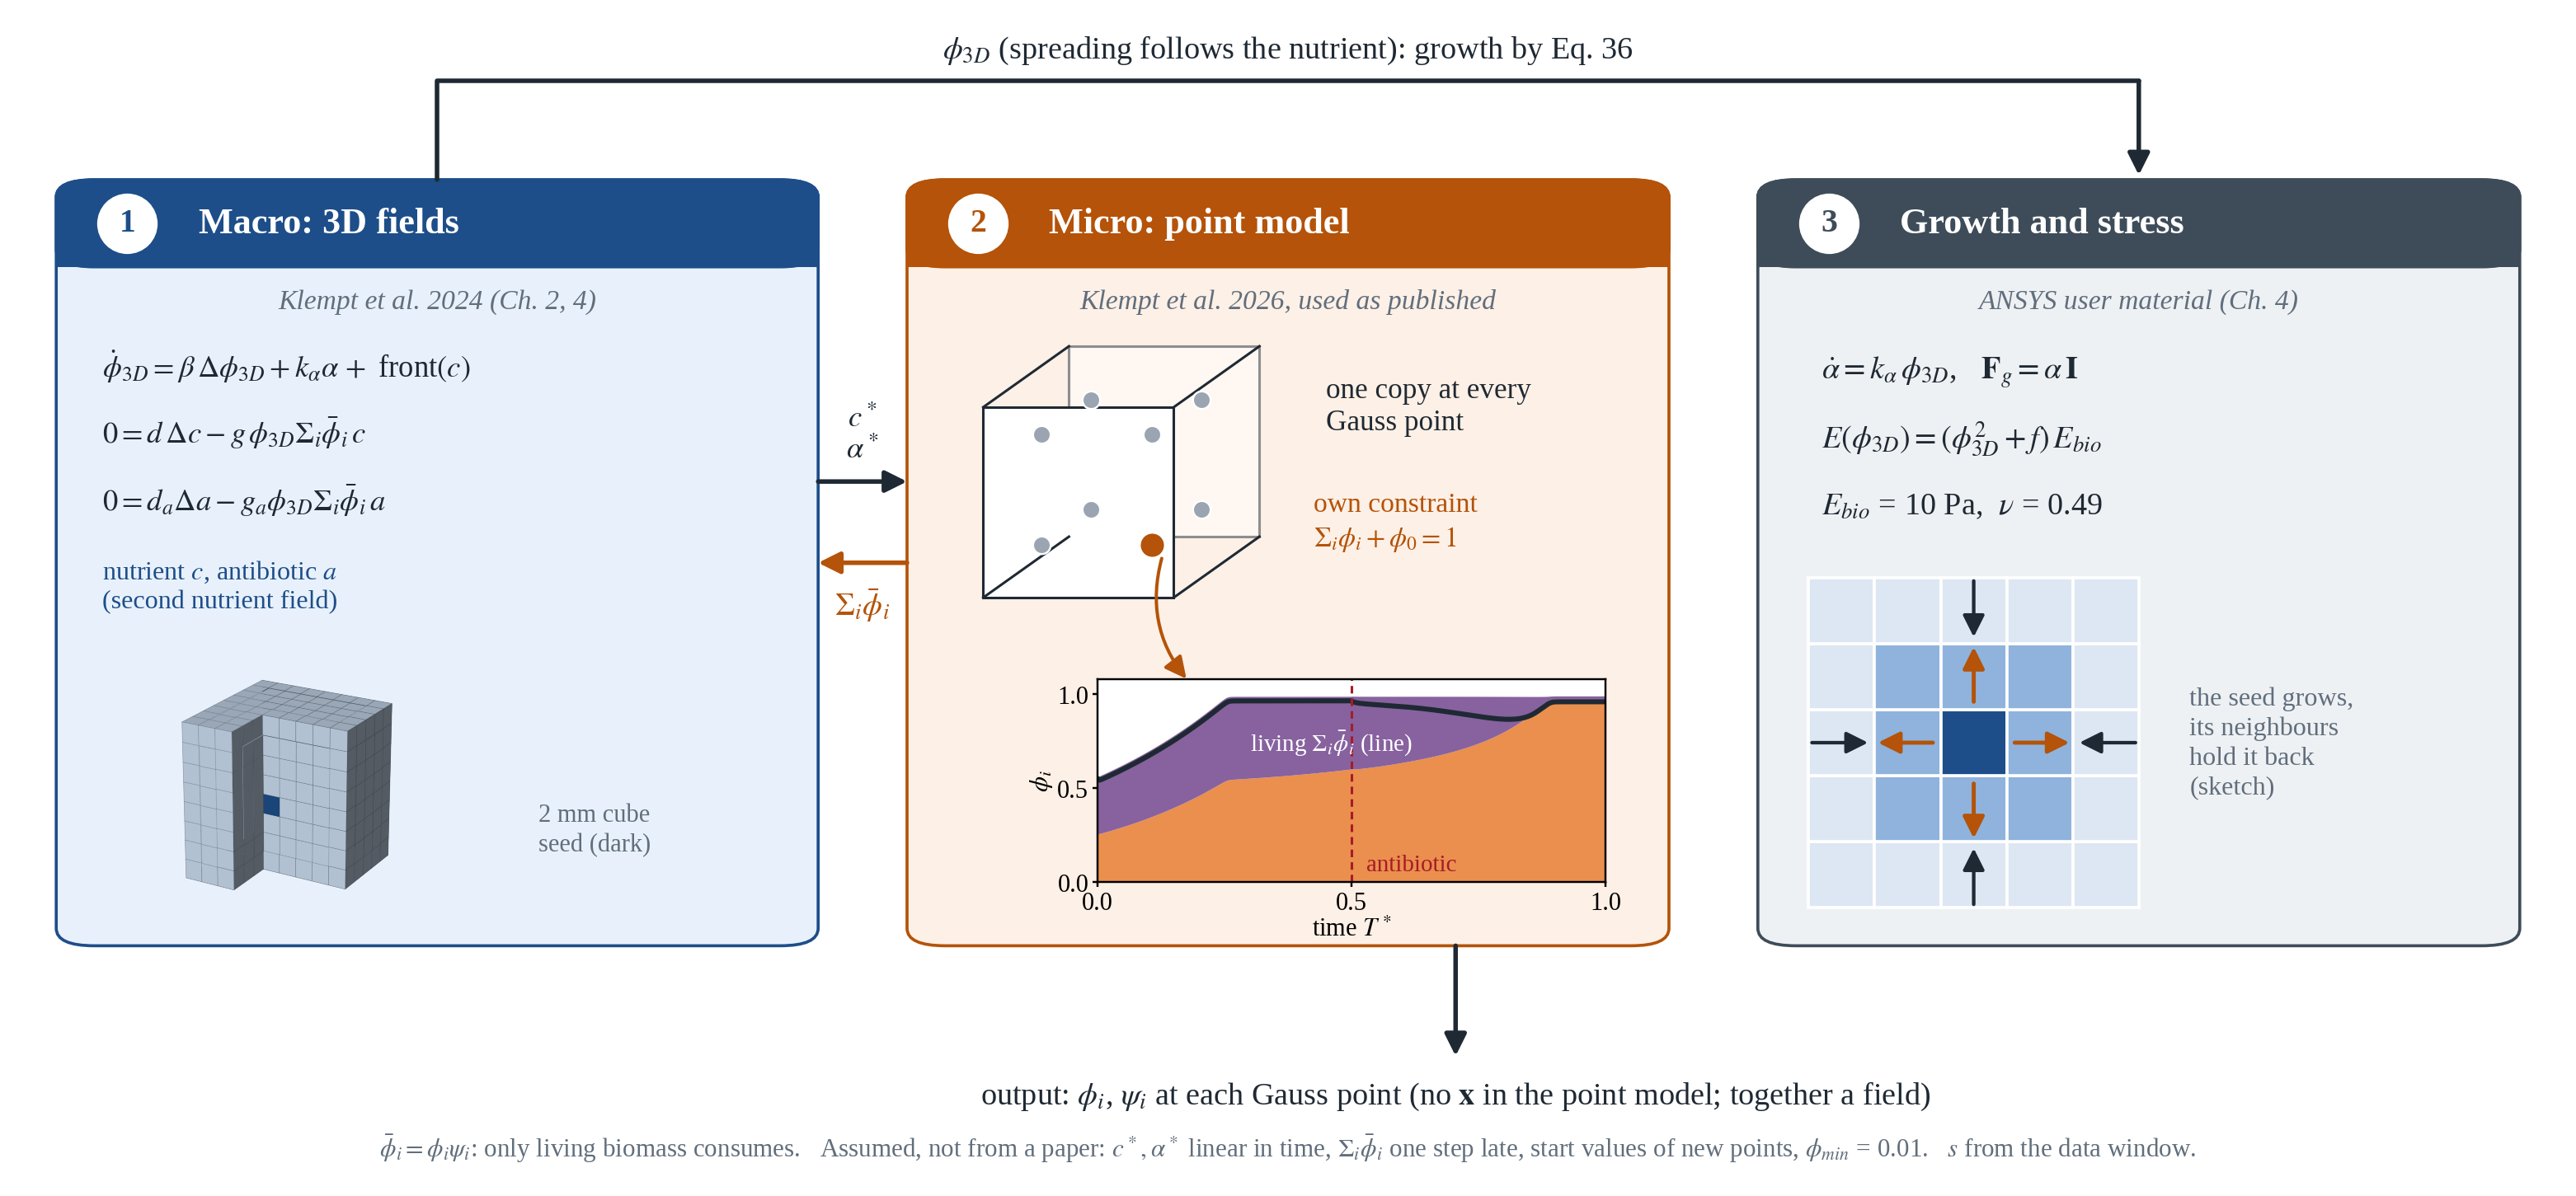
\includegraphics[width=0.92\linewidth,height=0.6\textheight,keepaspectratio]{fig_coupling_schematic_agreed.png}
\begin{itemize}\small
  \item 点モデル（Klempt et al.\ 2026）を論文どおり，各 Gauss 点で動かします．
  \item 栄養 $c$ と抗菌薬 $a$ を場から受け取り，生きている量 $\sum_i\bar\phi_i$ だけがそれを消費します．
\end{itemize}
\end{frame}

% --------------------------------------------------------
\begin{frame}{結果：2菌種と抗菌薬}
\centering
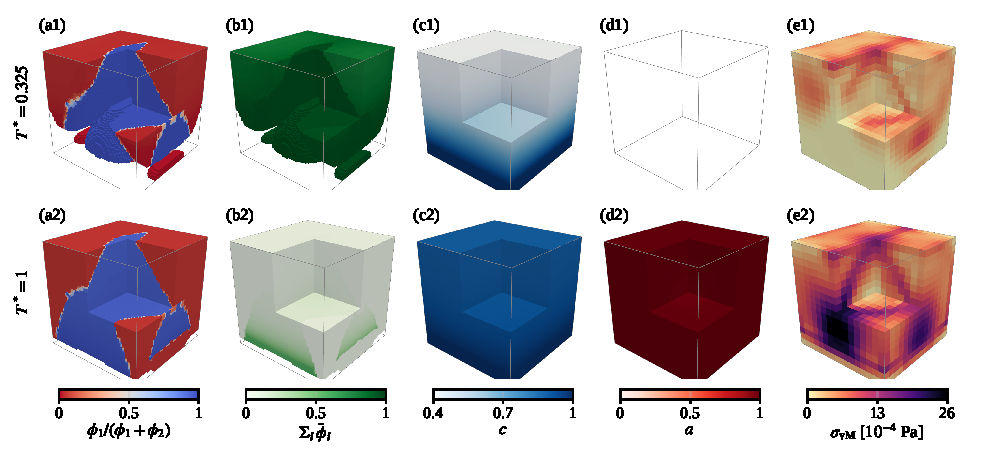
\includegraphics[width=0.74\linewidth]{fig_coupled_3d_panels_separate_ab.pdf}\\[2pt]
{\scriptsize 分けて置いた例，抗菌薬あり．上 $T^*=0.325$，下 $T^*=1$：A の割合，$\sum_i\bar\phi_i$，$c$，$a$，von Mises 応力．}
\begin{itemize}\small
  \item 合成データ（Fritsch et al.\ 2025，case I）と論文の定数．抗菌薬は $T^*=1/3$ から．
  \item シードの生きている量：分けて置くと $0.96\to0.15$，混ぜて置くと $0.96\to0.04$．成長はほぼ変わりません．
\end{itemize}
\end{frame}

% --------------------------------------------------------
\begin{frame}{検証：格子収束と前線の項 $-r\tfrac{c}{k+c}\,\mathbf n_c\cdot\nabla\phi_{3D}$}
\begin{columns}[T]
\column{0.55\textwidth}
\small シードの平均，抗菌薬あり，$T^*=1$（Python，$32^3/64^3/128^3$）\\[4pt]
\begin{tabular}{llcc}
\toprule
例 & 量 & 外挿値 & GCI \\
\midrule
分けて置く & $\alpha-1$ & $9.22\times10^{-4}$ & 1.5\,\% \\
分けて置く & von Mises & $6.7\times10^{-4}$~Pa & 8\,\% \\
混ぜて置く & $\alpha-1$ & $8.54\times10^{-4}$ & 3.3\,\% \\
混ぜて置く & von Mises & $4.0\times10^{-4}$~Pa & 26\,\% \\
\bottomrule
\end{tabular}
\column{0.43\textwidth}
\small
\begin{itemize}\setlength{\itemsep}{4pt}
  \item 前線の項 $-r\tfrac{c}{k+c}\,\mathbf n_c\cdot\nabla\phi_{3D}$ はセルのペクレ数が約31（$16^3$）．一定の人工拡散では応力が4分の1になります．
  \item 2次の風上差分なら成長と組成は数\,\%で収束し，応力は遅く収束します．
  \item IKM の要素（ANSYS）も同じ式を解き，この幅に入ります．
\end{itemize}
\end{columns}
\end{frame}

% --------------------------------------------------------
\begin{frame}{ご相談1：来年の学会発表}
\begin{columns}[T]
\column{0.5\textwidth}
\textbf{USNCCM19}（米国計算力学会議）
\begin{itemize}\small
  \item 2027年7月25〜29日，パサデナ（ロサンゼルス近郊）
  \item 抄録 2026年11月16日〜2027年1月15日
  \item 学生の旅費の助成 2027年1月1日〜3月31日
  \item 内容：バイオフィルムの連成と検証（IKM と共著．10月26日に Soleimani 先生へ許可を伺うメールを送付，返事待ち）
\end{itemize}
\column{0.46\textwidth}
\textbf{SQAI-NCTS}（台湾，8月）
\begin{itemize}\small
  \item 量子機械学習の発表（予定どおり）
\end{itemize}
\vspace{6pt}
\textbf{伺いたいこと}
\begin{itemize}\small
  \item 研究室で USNCCM19 に行く予定はありますか．
  \item 慶應の所属の書き方，先生に共著に入っていただけるか．
  \item 旅費の扱い．
\end{itemize}
\end{columns}
\end{frame}

% --------------------------------------------------------
\begin{frame}{ご相談2：4月からの RA}
\begin{itemize}\setlength{\itemsep}{6pt}
  \item IKM の HiWi は 2027年3月末まで延長になりました（Junker 先生）．
  \item 2027年4月から週20時間ほど，RA としてお手伝いできればと思います．
  \item JAXA，量子機械学習，CFRP の NEDO の件に限らず，研究室のほかのプロジェクトでも構いません．
  \item できること：FEM（ANSYS のユーザー要素，Abaqus），JAX での高速化，ベイズ推定（TMCMC），GNN，論文の図と英語の校正．
  \item 研究室で難しい場合は，共同研究先などで有給の仕事があればご紹介いただけると助かります．
  \item 就職活動は3月で終わる予定です．
\end{itemize}
\end{frame}

% --------------------------------------------------------
\begin{frame}{ご相談3：課題研究報告と慶應での修士論文}
\begin{columns}[T]
\column{0.48\textwidth}
\textbf{課題研究報告}（2027年3月12日 16:00 締切）
\begin{itemize}\small
  \item LUH の修士論文をもとに書いてよいか．
  \item 共著の論文がある場合の扱い（単著の規定）．
\end{itemize}
\vspace{6pt}
\textbf{論文}
\begin{itemize}\small
  \item TMCMC の論文：近く投稿します．
  \item 連成の論文：2027年3〜4月に投稿，12月の発表までに掲載を目指します．
\end{itemize}
\column{0.48\textwidth}
\textbf{慶應での修士論文}（2028年3月修了）
\begin{itemize}\small
  \item テーマはバイオフィルムの続きでよいか．
  \item 候補：応力から成長への戻り（Klempt 2024 の Eq.~30 が落とした項），5菌種を要素へ，Abaqus での実装．
  \item 帰国後の環境：研究室の席，PC と GPU，Abaqus のライセンス．
\end{itemize}
\end{columns}
\end{frame}

% --------------------------------------------------------
\begin{frame}{慶應での研究計画：本命の論文（2027年9月投稿）}
\begin{columns}[T]
\column{0.5\textwidth}
\small
\textbf{内容}：圧力で成長が止まる成長則
\[
\dot\alpha=k_\alpha\phi\,\max\bigl(0,\,1-p/p_h\bigr)
\]
を持つバイオフィルムの連続体モデルを，較正した組成と一緒にインプラント・歯の形で解く（Abaqus のユーザー要素）．
\vspace{4pt}

\textbf{できていること}
\begin{itemize}\footnotesize
  \item 成長則の検証（自由成長・全拘束，接線は差分と $4\times10^{-10}$）
  \item 扇形のメッシュ収束（3 段）
  \item 歯頸線：成長則なしでは歯頸線に応力が集中（比 1.37），$p_h<p_0$ なら集中が消える（比 0.67）
\end{itemize}
\textbf{残り}：Abaqus 本体での確認，文献・実験との比較，DS・DH の組成
\column{0.48\textwidth}
\centering
\includegraphics[width=\linewidth]{fig_cervical.pdf}\\
{\scriptsize 歯頸線の帯の応力（コアとの比，3 段のメッシュ）}
\vspace{4pt}
\begin{itemize}\footnotesize
  \item \textbf{伺いたいこと}：比べられる実験（研究室の測定，共同研究先），投稿先（BMMB，JMBBM など）
\end{itemize}
\end{columns}
\end{frame}

% ========================================================
\appendix
\begin{frame}{付録：記号と式}
\small
\begin{tabular}{ll}
\toprule
$\phi_{3D}$，$\alpha$ & バイオフィルムの量と成長（$\mathbf F_g=\alpha\mathbf I$，$\alpha(0)=1$，成長は $\alpha-1$） \\
$c$，$a$ & 栄養と抗菌薬の場 \\
$\phi_i$，$\psi_i$，$\phi_0$ & 菌種 $i$ の体積分率と生存率，空隙（Klempt et al.\ 2026）\\
$\bar\phi_i=\phi_i\psi_i$ & 菌種 $i$ の生きている体積分率 \\
$c^*=c^*_0c$，$\alpha^*=\alpha^*_0a$ & 点モデルが見る栄養と抗菌薬 \\
\bottomrule
\end{tabular}
\begin{align*}
\dot\phi_{3D}&=\beta\nabla^2\phi_{3D}+k_\alpha\alpha-r\tfrac{c}{k+c}\,\mathbf n_c\cdot\nabla\phi_{3D} &&\text{（Eq.~34，前線の項あり）}\\
\dot c&=d\nabla^2c-g\,\phi_{3D}\textstyle\sum_i\bar\phi_i\,c,\quad \dot a=d\nabla^2a-g\,\phi_{3D}\textstyle\sum_i\bar\phi_i\,a &&\text{（Eq.~35）}\\
\dot\alpha&=k_\alpha\phi_{3D} &&\text{（Eq.~36）}
\end{align*}
定数は Klempt et al.\ 2024 の Table 2 を 2~mm の立方体に換算（$\beta$ の換算は仮定）．
\end{frame}

\end{document}
